%%%%%%%%%%%%%%%%%%%%%%%%%%%%%%%%%%%%%%%%%
% Twenty Seconds Resume/CV
% LaTeX Template
% Version 1.0 (14/7/16)
%
% This template has been downloaded from:
% http://www.LaTeXTemplates.com
%
% Original author:
% Carmine Spagnuolo (cspagnuolo@unisa.it) with major modifications by 
% Vel (vel@LaTeXTemplates.com) and Harsh Gadgil
%
% License:
% The MIT License (see included LICENSE file)
%
%%%%%%%%%%%%%%%%%%%%%%%%%%%%%%%%%%%%%%%%%

%----------------------------------------------------------------------------------------
%    PACKAGES AND OTHER DOCUMENT CONFIGURATIONS
%----------------------------------------------------------------------------------------

\def\zh_CN_CV{0}

%\documentclass[letterpaper]{twentysecondcv} % a4paper for A4
\documentclass[utf8]{twentysecondcv} % a4paper for A4
%\usepackage[utf8]{inputenc}

% Command for printing skill progress bars
\newcommand\skills{ 
~
    \smartdiagram[bubble diagram]{
        \textbf{Self-motivated}\\\textbf{Dev},
        \textbf{Relational/}\\\textbf{Document}\\\textbf{DB},
        %\textbf{~~~~OOP~~~~~},        
        \textbf{Latex/}\\\textbf{Markdown},
        \textbf{Web}\\\textbf{Stuff},
        \textbf{Machine}\\\textbf{Learning},
        \textbf{Deep}\\\textbf{Learning},
        \textbf{Hardware}\\\textbf{Programming},
        \textbf{Computer}\\\textbf{Vision}
    }
}

%\interests{{Functional Programming/4.5},{ML DL/5},{Software Engineering/6},{Computer Vision/6}}
% Programming skill bars
\programming{{Java $\textbullet$ JS $\textbullet$ HTML / 3.5}, {C++ $\textbullet$ C  $\textbullet$ Arduino / 4.5},  {OpenCV $\textbullet$ Python $\textbullet$ Markdown / 6}}


% Projects text
\experience{
\textbf{TJU RM Member} \\ CV, DL methods on object detection, tracking and decision making. \\
        \textbf{Teaching Assistant} \\ Programming Design Practice I, full English course for freshmen. \\
        \textbf{Teaching Python101} \\ Teaching python for several overseas master candidates major in finance. \\
        \textbf{Valunteer Teacher} \\ Volunteered to teach in a primary school in TongChuan, Shannxi, organized by “Dripping Action”(one project of Mutualistic Symbiosis Community of Youths \& Environment, Shaanxi).
        %\textbf{Club activities} - Member of Young Volunteer team and Work-study centre clubs in Xidian.
}


%----------------------------------------------------------------------------------------
%     PERSONAL INFORMATION
%----------------------------------------------------------------------------------------

% If you don't need one or more of the below, just remove the content leaving the command, e.g. \cvnumberphone{}



\cvname{{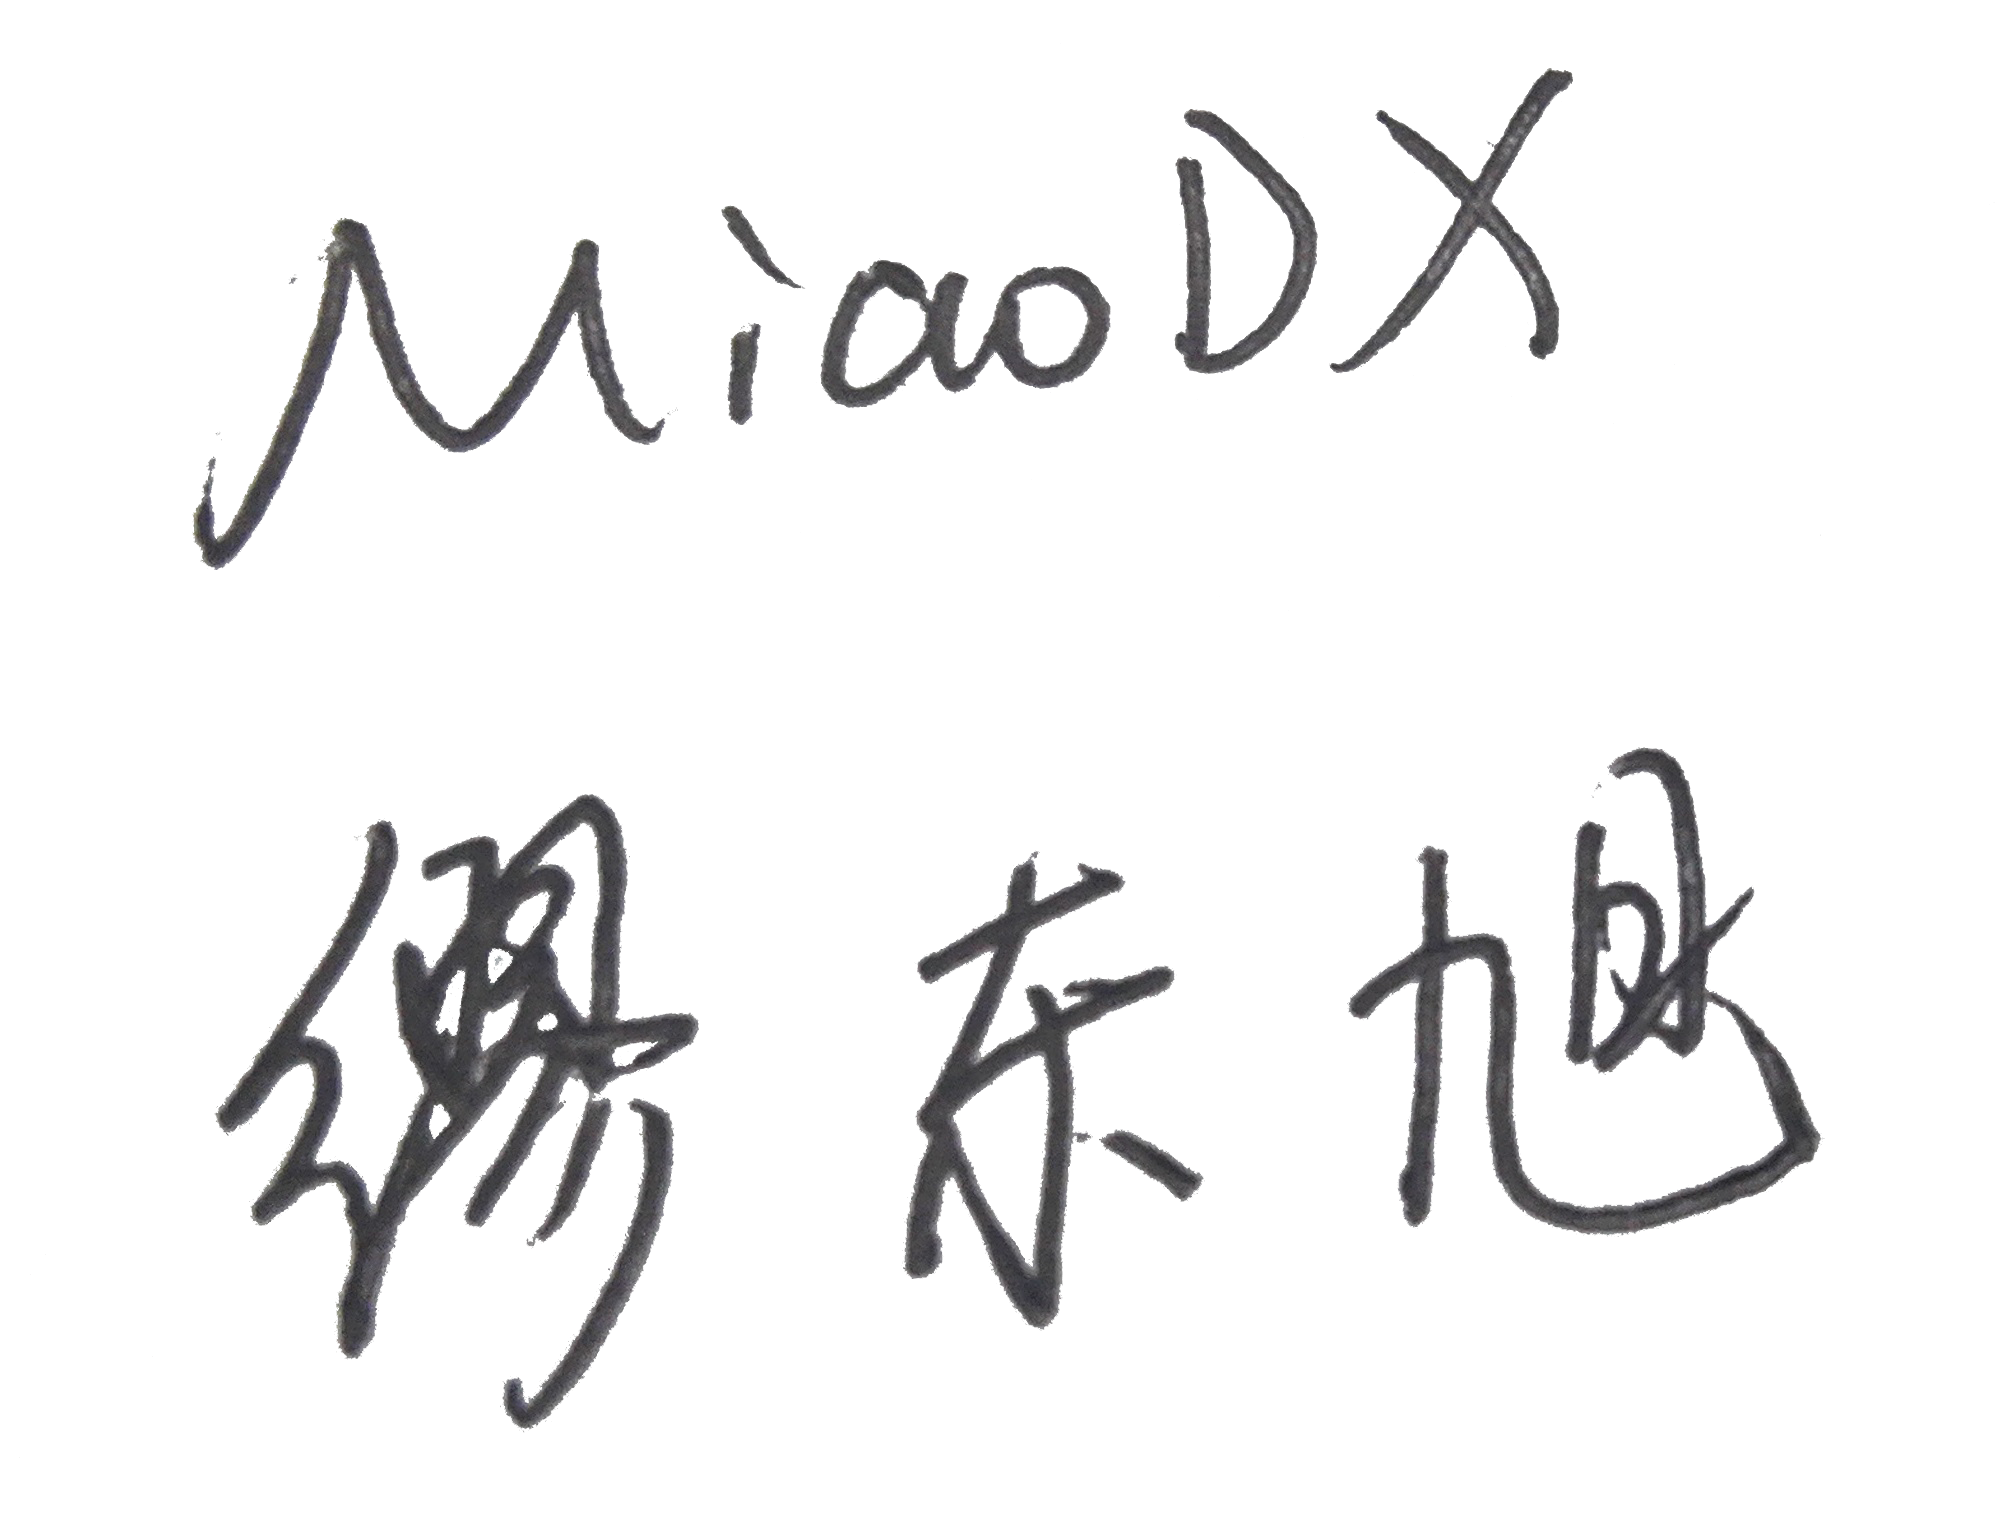
\includegraphics[scale=0.04]{img/miaodx_name.png}}} % Your name
\cvjobtitle{ Graduate Student, \\ Self-motivated Developer} % Job title/career

%\cvlinkedin{https://linkedin.com/in/miaodx}
\cvgithub{https://github.com/MiaoDX}
\cvnumberphone{+86 13502009660} % Phone number
\cvsite{https://miaodx.github.io/} % Personal website
\cvmail{miaodx@tju.edu.cn} % Email address

%----------------------------------------------------------------------------------------

\begin{document}

\makeprofile % Print the sidebar

%----------------------------------------------------------------------------------------
%     EDUCATION
%----------------------------------------------------------------------------------------
\section{Education}

\begin{twentyshort}
    \twentyitemshort
        {2016 - Now}
        {MSe., Computer Software \hfill{Tianjin University}}	
	\twentyitemshort
		{2012 - 2016}
		{BEng., Computer Software \hfill{Xidian University}}		
\end{twentyshort}


%\begin{twenty} % Environment for a list with descriptions
%    \twentyitem
%        %{Expected \\ Dec 2016}
%        {2016 - Now}
%        {}
%        {MSe., Computer Software}
%        {\href{http://tju.edu.cn/}{Tianjin University}}
%        {Tianjin, China}
%        {\vspace{-10pt}}
%    \twentyitem
%        {2012 - 2016}
%        {}
%        {BEng., Computer Software}
%        {\href{http://www.xidian.edu.cn/}{Xidian University}}
%        {Xi'an, Shaanxi, China}
%        {\vspace{-10pt}}
%    %\twentyitem{<dates>}{<title>}{<organization>}{<location>}{<description>}
%\end{twenty}



\section{Scholarships \& Awards}

\begin{twentyshort}
    \twentyitemshort
        {2017-2018}
        {Second-class School Scholarship}
	\twentyitemshort
        {2016-2017}
        {First-class School Scholarship}
	\twentyitemshort
		{Oct 2016}        
		{Postgraduate recommendation offer from Tianjin University}
	\twentyitemshort
		{2014-2015}
		{National Inspiration Scholarship}
	\twentyitemshort
		{2014CUMCM}
		{Second-class prize in Shaanxi Division}
	\twentyitemshort
		{2013-2014}
		{Second-class School Scholarship}		
	\twentyitemshort
		{2012-2013}
		{First-class School Scholarship}		
\end{twentyshort}        


\section{Papers}

\begin{twenty}
    \twentyitem
        {Jan 2018}
        {}        
        {Paper Accpeted by ICASSP 2018}
        {}
        {}
        {ACTIVE CAMERA RELOCALIZATION WITH RGBD CAMERA
FROM A SINGLE 2D IMAGE (Camera ready, First Author)}
    \twentyitem
        {Mar 2018}
        {}        
        {Paper Accpeted by ICME 2018}
        {}
        {}
        {Fast and Reliable Computational Rephotography on Mobile Device (Camera ready, Oral, Third Author)}
\end{twenty}

\section{Projects}
\begin{twenty}

    \twentyitem
        {}
        {}        
        {Recent projects, more can be found on github}
        {\href{https://github.com/MiaoDX/}{github.com/MiaoDX}}
        {}
        {}
          
    \twentyitem
    {Jan 2018 - }
    {May 2018}
    {ICRA 2018 DJI ROBOMASTER AI CHALLENGE}
    {}
    {}
    {Took part in ICRA 2018 DJI RM AI CHALLENGE with other five teammates from TJU. In charge of object detection and tracking. Got the finalist invitation.}
    
    \twentyitem
    {Mar 2016 -}
    {Present}
    {Active Camera Relocalization}
    {}
    {}
    {Actively relocate camera to previous pose is one fundamental research area in robotics and computer vision. Major part of my undergraduate graduation and conference papers.}
    
	\twentyitem
        {Python}
		{Data Label}
        {Data Labelling tool for ML/DL}
        {\href{https://github.com/MiaoDX/DataLabel}{DataLabel}}
        {}
        {Data labelling tool to make the work less tedious with tracking methods underneath. Export file for DLIB and Darkflow.}
          
    \twentyitem
        {Virtual Env}
      	{DL}
        {UnrealCV with Deep Learning (Faster-RCNN)}
        {\href{https://github.com/MiaoDX/unrealcv_examples/}{UnrealCV \& DL}}
        {}
        {Integrate (\href{https://github.com/smallcorgi/Faster-RCNN\_TF}{smallcorgi/Faster-RCNN\_TF}) with virtual environment library \href{https://github.com/unrealcv/unrealcv}{UnrealCV}. Exploring the potential benefits of synthetic data on improving exisiting DL implements.}
                 
    \twentyitem
        {Python}
		{RL}
        {PacMan capture the flag with Reinforcement Learning}
        {\href{https://github.com/MiaoDX/hand_in_homework/tree/master/Advanced\_AI/}{PacMan \& RL}}
        {}
        {Some reinforcement projects on pacman capture the flag game, with fundamental concepts and a contest hold in class.}
        
		\twentyitem
        {OpenCV}
        {Flask}
        {Restful depth camera}
        {\href{https://github.com/MiaoDX/depth\_camera}{Depth\_camera \& http}}
        {}
        {Expose one stereo camera (ZED) into restful one, so that it can be accessed from other programming languages with ease.}

	    \twentyitem
        {Python}
		{ML}
        {UCI Adult database processing with scikit-learn}
        {\href{https://github.com/MiaoDX/scikit\_learning/}{scikit\_learning}}
        {}
        {Use sklearn to predict whether income exceeds \$50K/yr based on census data, got best result in class (85\%+ precision).}
        
        \twentyitem
        {Java}
       	{BP}
        {Back propagation implementation using java}
        {\href{https://github.com/MiaoDX/bp_java}{BP\_java}}
        {}                
        {It helped a lot to understand DL by implementing one simple ANN from scratch before diving into those amazing open source ML(\/DL) libraries.}
		
		\twentyitem
        {Node.js}
        {MongoDB}
        {Attendance management system}
        {\href{https://github.com/SEAPC2016/attendance}{Attendance system}}
        {}
        {In a team of four, made an RESTful attendace webset system with Node.js, mongodb and Jade for a (faked) company. Stuffs can ask for leave via our system and wait for the managers's approval, statistical information can also be generated from our system.}


\end{twenty}





%\begin{twenty}

%    \twentyitem
%        {OpenCV}
%        {Notes on OpenCV}
%        {\href{https://github.com/MiaoDX/opencv\_projects/}{opencv\_notes}}
%        {}
%        {Notes, example codes and some tricks for working with OpenCV.}

%    \twentyitem
%        {Baidu Map API  \\ D3.js}
%        {Display churches in Tianjin}
%        {\href{https://github.com/MiaoDX/baidu\_map\_church}{baidu\_map\_church}}    
%        {}
%        {Course project of Visual Analysis class, since I really love the architecture of old churches, so I use Baidu Map API to get all churches' locations in Tianjin and display them with D3.js.}    
%\end{twenty}














%\section{Experience}
%
%\begin{twenty}
%
%\twentyitem
%    {June 2017 -}
%    {Now}
%    {Member of TJU RM}
%    {\href{http://tju.edu.cn/}{Tianjin University}}
%    {}
%    {Member of algorithm group, Tianjin University DJI Robomaster team, be responsible for computer vision, deep learning methods on object detection, tracking and decision making.}
%
%
%
%\twentyitem
%    {Feb 2017 -}
%	{July 2017}
%    {Graduate Teaching Assistant}
%    {\href{http://tju.edu.cn/}{Tianjin University}}
%    {}
%    {TA for Programming Design Practice I, full English course for freshmen.}    
%
%\twentyitem
%    {Feb 2017 -}
%   	{May 2017}
%    {Teaching Python101}
%    {\href{https://github.com/MiaoDX/python101}{MiaoDX/python101}}
%    {}
%    {Teaching python for several master students major in finance for their preparing for overseas study.}    
%
%\twentyitem
%    {Summer vacation}
%    {2013}
%    {Valunteer Teacher}
%    {\href{http://blog.sina.com.cn/xiaanedu}{Dripping Action}}
%    {}
%    {I volunteered to teach in a primary school in TongChuan, Shannxi province for more than half a month(18 days) with my teammates, that volunteer work was organized by “Dripping Action”(one project of Mutualistic Symbiosis Community of Youths \& Environment, Shaanxi).
%    }
%
%
%\twentyitem
%    {Sep 2012 -}
%  	{Sep 2013}
%    {Undergraduate club activities}
%    {\href{http://www.xidian.edu.cn/}{Xidian University}}
%    {}
%    {Member of Young Volunteer team and Work-study centre clubs in
%School.}    
%
%
%    
%    
%\end{twenty}
%
%\section{Personal}
%
%\begin{twenty} % Environment for a list with descriptions
%    
%\twentyitem
%    {}
%    {}
%    {}
%    {}
%    {}
%    {        
%        {\begin{itemize}
%            \item Passed CET-6 (460), English as working language
%            \item Reading, Boxing, Running, Cycling          
%        \end{itemize}
%         }
%    }    
%        
%    %\twentyitem{<dates>}{<title>}{<location>}{<description>}
%\end{twenty}

\end{document} 
